\section{Design Overview}

% Boost Stage
\subsection{Boost Stage}
Since the SFRJ should be launched using an off-the-shelf solid rocket motor, the design team selected the most powerful motor that could be acquired. The Cesaroni Pro150 come in three options, each with a different casing size, impulse, and burn duration. Ultimately, the Pro150-40960O8000 variant was selected for the highest total impulse \cite{cesaroni}. The specifications for the O8000 motor are provided in Table \ref{tab:cesaroniSpecs}. The booster would need to launch as large a payload as possible to around Mach 2-2.5, and further details on the trade performed can be found in the Trade Study section of this report.

\begin{table}[H]
    \centering
    \caption{Cesaroni Pro150-40960O8000-P Booster Specs \cite{cesaroni}}
    \begin{tabular}{c|c}
    \textbf{Parameter} & \textbf{Value} \\
    \hline
         Length & 37.68 in \\
         Diameter & 6.34 in \\
         Impulse & 9206 $\text{lb}_{\text{f}}$*s \\
         Burn Time & 5.12 s \\
         Specific Impulse & 224.4 s \\
         Total Booster Weight & 71.47 lb \\
         Propellant Weight & 40.71 lb \\
         Burnout Weight & 29.48 lb \\
    \end{tabular}
    \label{tab:cesaroniSpecs}
\end{table}

% Solid Fuel Ramjet Stage
\subsection{Solid Fuel Ramjet Stage}
\color{red}Insert CAD, mass breakdowns.\color{black}

\begin{table}[H]
\centering
\caption{SFRJ Mass Breakdown}
\label{tab:masses}
\begin{tabular}{l|c|c}
\textbf{Sub-Assembly} & \textbf{Mass [lb (kg)]} & \textbf{Percent of Total} \\
\hline
Inlet & 5.99 (2.72) & 10.24\% \\
GNC & 5.99 (1.82) & 6.87\% \\
Fuel & 4.02 (4.66) & 17.57\% \\
Combustor & 10.28 (8.38) & 31.57\% \\
Fins and Actuators & 6.24 (2.83) & 10.66\% \\
Nozzle & 2.18 (0.99) & 3.73\% \\
AeroValve & 7.33 (3.32) & 12.53\% \\
Airframe & 4.00 (1.81) & 6.84\% \\
\hline
TOTAL & 58.51  (26.54) & 100\% \\
\end{tabular}
\end{table}

\subsubsection{Key Features - Silas Meriam}
Insert exploded components graphic, and description of aerovalve.

\subsubsection{Concept of Operations - Thomas Satterly and Melanie Grande}
The concept of operations for the GLD (illustrated in Fig. \ref{fig:trajectoryOverview}) was defined to create a baseline design and develop further performance requirements for the system. The mission begins with launch at a constant elevation angle using the Cesaroni Pro150 boost stage. After booster burnout and separation, the SFRJ pitches to level flight. During cruise, the SFRJ flies near Mach 2 for adequate stagnation pressure and temperature. Additionally, the stage will make two 45\textdegree yaw maneuvers--followed by 90-180\textdegree rolls in the direction of the desired turn--during its approximately 30 second burn.

\begin{figure}[H]
    \centering
    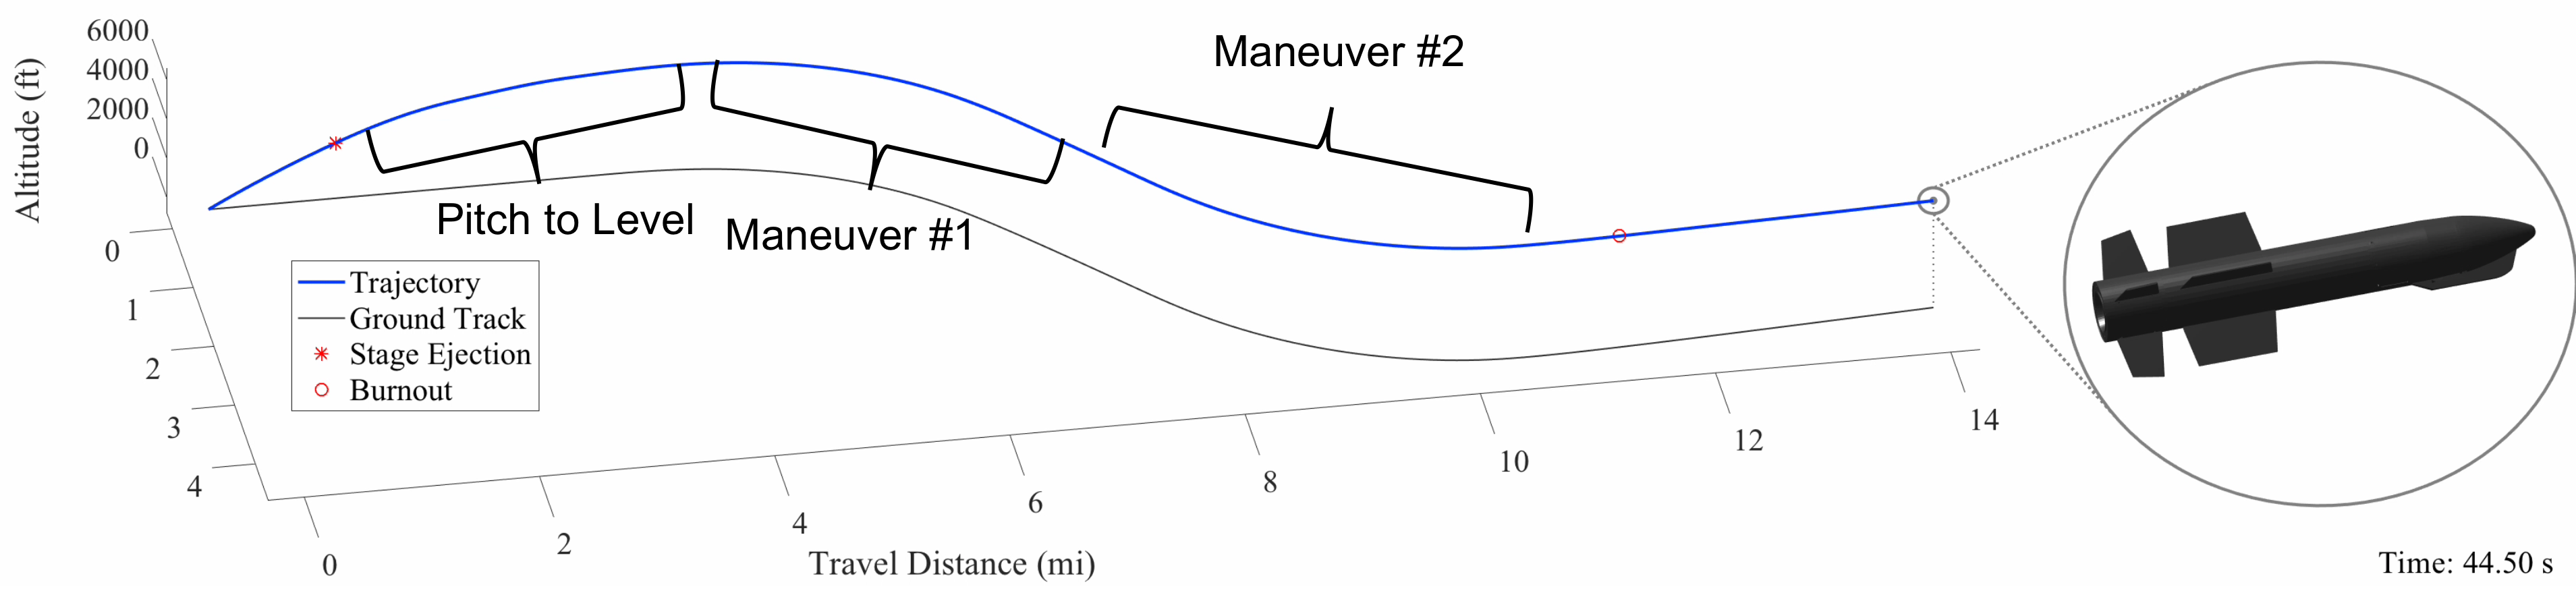
\includegraphics[width=\textwidth]{OverviewFigures/TrajectoryOverview.png}
    \caption{Trajectory overview of SFRJ and boost stages.}
    \label{fig:trajectoryOverview}
\end{figure}

\subsubsection{Performance Summary - Thomas Satterly}

The SFRJ has a predicted burn time of 27.3 seconds, providing 11.9 miles of total range. Additional performance figures are provided in Table \ref{tab:PerformanceOveriew}. In comparison, the currently deployed AIM-9 missile, which has a slightly smaller diameter but is twice the length and three times the mass, has a maximum ground range of 22 miles. This is roughly twice the range of the SFRJ, but at the expense of three times the total mass. The Cesaroni Pro-150 solid rocket booster is also comparable. The booster has a slightly greater initial mass but four times the fuel mass versus the SFRJ, but delivers slightly less total impulse. In both comparisons, the proposed SFRJ design offers arguable better performance than existing systems, suggesting that future investigation with physical demonstrators is a worthwhile endeavor. 

\begin{table}[H]
\centering
\caption{SFRJ Performance Overview and Comparison}
\label{tab:PerformanceOveriew}
\begin{tabular}{l|c|c|c}
& \textbf{SFRJ} & \textbf{AIM-9} & \textbf{Cesaroni Pro 150}\\
\hline
Total Length & 48.5 in (1.23 m) & 119 in (3 m) & - \\
Grain Length & 21.65 in (0.55 m) & - & - \\
Diameter & 6.3 in (0.16 m) & 5 in (0.127 m) & - \\
Initial Mass & 58.51 lbs (26.54 kg) & 188 lbs (85.28 kg) & 71.47 lbs (32.42)\\
Propellant Mass & 10.3 lbs (4.7 kg) & - & 40.7 lbs (18.6 kg) \\
Average Thrust & 339.5 $\text{lb}_{\text{f}}$ (1.5 kn) & - & 1807 $\text{lb}_{\text{f}}$ (8.03 kN) \\
Average Freestream Mach & 2.1 & 2.5+ & - \\
Burn Time & 27.3 s & - & 5.12 s\\
Average $\text{Isp}_{\text{f}}$ (HTPB Fuel) & 1056.7 s & - & - \\
Total Impulse & 9268.4 $\text{lb}_{\text{f}}$*s (41 kN*s) & - & 9216 $\text{lb}_{\text{f}}$*s (40.96 kN*s)\\
Ground Range & 11.9 mi (19.2 km) & 22 mi (35.4 km) & - \\
Payload Mass Percentage & 5\% & 10\% & -
\end{tabular}
\end{table}